\clearpage
\begin{lrbox}{\methodologyoverviewbox}
\begin{minipage}{\linewidth}
\section{Methodology}
\label{sec:methodology}

Figure~\ref{fig:architecture} shows how the seven GRASP modules connect company BRSR reports with analysis and sector comparisons. Text segments and reported figures are stored together in a database. Labelled text segments are used to train the BERT principle classifier, while language and numerical checks identify disclosures for review. The Transparency Score combines Completeness, Specificity, Clarity, and mapped Sustainable Development Goal coverage to support company comparisons. The service layer provides access to these results through an application programming interface (API). Principle probabilities, claim--figure review records, and Transparency Scores are provided as separate outputs.

\par\medskip
{\centering
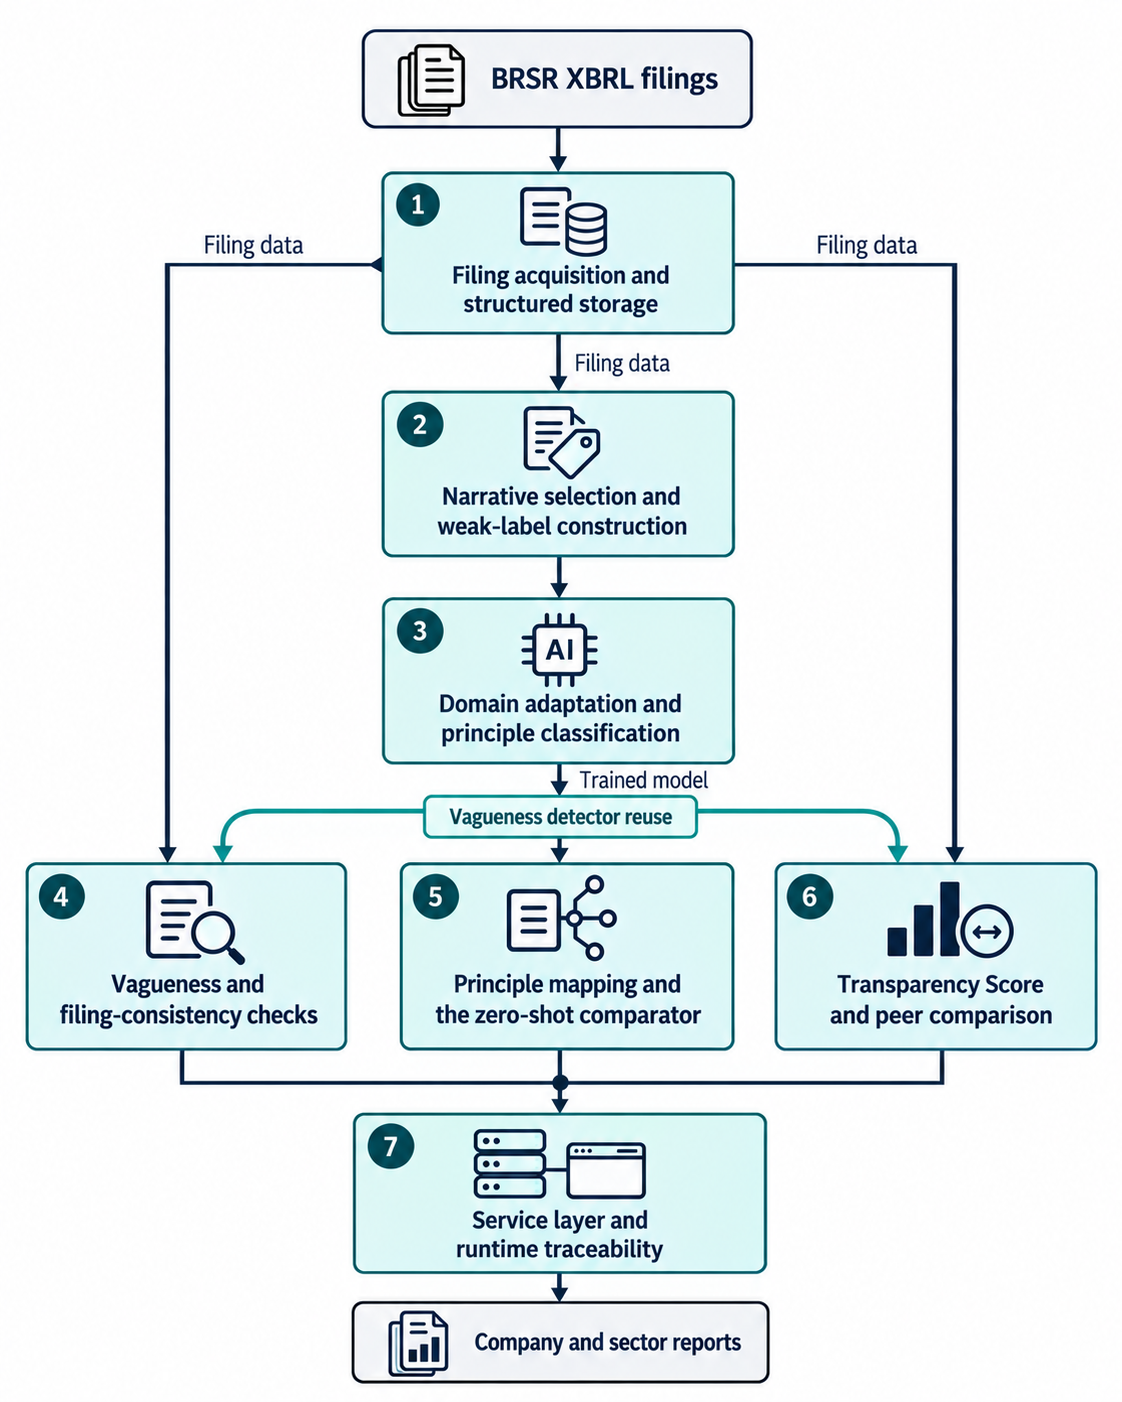
\includegraphics[width=0.98\linewidth,height=0.72\textheight,keepaspectratio]{figures/grasp_pipeline.png}
\captionof{figure}{This figure shows the overall workflow of GRASP and how the main components connect to support BRSR report analysis.}
\label{fig:architecture}
\par}

\end{minipage}
\end{lrbox}
\ifdim\dimexpr\ht\methodologyoverviewbox+\dp\methodologyoverviewbox\relax>\textheight
\PackageError{GRASP-layout}{Methodology overview exceeds one page}{Reduce the diagram height.}
\fi
\noindent\usebox{\methodologyoverviewbox}
\par\clearpage

\subsection{Filing acquisition and structured storage}
\label{sec:ingestion}

The input consists of BRSR filings in eXtensible Business Reporting Language (XBRL), together with company identifiers. A download log records completed and failed files so collection can resume after an interruption. The parser reads structured filing data directly. A concept names a reporting item, such as water withdrawal. The context records the company, period, and any reporting categories, while the unit records how a numerical value is measured \cite{xbrl2013}. This structure keeps a figure linked to the information needed for comparison.

The database has three linked record types. A company record stores the Corporate Identity Number (CIN), name, and industry code. A filing record stores the company link, reporting dates, and source location. A fact record stores the concept, original value, unit, stated precision when available, period, and dimensions. Dimensions are categories such as gender or employment type. A workforce count can therefore retain these categories instead of becoming one combined number. Values are stored as text and converted to numbers only when a calculation requires arithmetic. A company--year uniqueness rule limits duplicate ingestion of the same filing.

The output is a searchable database of reported facts. Each value retains a link to the source filing, reported concept, period, and unit. These links support later passage review, numerical comparison, and company-score calculation.

\subsection{Narrative selection and weak-label construction}
\label{sec:labels}

Text candidates come from concepts containing \artifact{ExplanatoryTextBlock}. Before counting words, the dataset builder removes URLs. At least 15 words of useful content must remain. Bare links, short fragments, and listed non-answers are removed. These rules define the classifier dataset. The company-scoring modules use different text-length rules, explained in Section~\ref{sec:score}. Classifier passages and scoring passages are therefore different groups of text.

Principle labels come from three sources, checked in order. An explicit \artifact{PrincipleAxis} tag supplies a Section B label. If that tag is unavailable, a Section C concept-to-principle map supplies the label. A numbered \artifact{NotesPrincipleX} concept provides the third source. The extension includes 29 AI-assisted assignments, with existing configured mappings taking priority when maps overlap. The process produces taxonomy-derived weak labels rather than independent passage-level expert judgements; the AI-assisted assignments have no completed independent expert verification.

Candidates are grouped by company, concept, and cleaned text. Repeated entries with the same label produce one row. A group with several labels is removed from the single-label dataset. These groups can include passages covering several principles or generic text reused under different questions. The resulting dataset contains 42,409 samples. The CSV records the label source for analysis, while only the passage text enters the classifier.

The labelled dataset is split by CIN. Training contains 29,834 passages from 814 companies, validation contains 6,374 passages from 175 companies, and test contains 6,201 passages from 175 companies. No company appears in more than one split. This company-based partition defines the main supervised evaluation. Exact wording shared across different companies is counted separately in the text-overlap check.

\subsection{Domain adaptation and principle classification}
\label{sec:classifier}

The encoder starts from \artifact{bert-base-uncased}. Masked language modelling adapts BERT to sustainability text: selected word pieces are hidden, and the model learns to predict the missing text. A nine-output classification layer is then added, and labelled training adjusts the model for the nine principles. For a passage $x$, the model returns a probability $p_k(x)$ for each principle $k$. The largest probability gives the Top-1 prediction. The two largest probabilities give the Top-2 candidate list \cite{devlin2019,gururangan2020}.

\paragraph{Model development and component roles.}
The final model follows four steps: base BERT, adaptation to BRSR text, supervised training for nine principles, and recovery of the selected seed-99 checkpoint. A checkpoint is a saved set of model parameters. Adaptation changes the parameters while keeping the BERT structure. Fine-tuning adds the classification output layer and updates the encoder. Recovery corrects saved parameter names and verifies loading without further training. MPNet supplies sentence similarity for vagueness checks and the zero-shot comparison. The final audited evaluation uses the recovered BERT classifier; earlier ClimateBERT and ensemble runs belong to the passage-level experiment history.

The classifier accepts at most 512 tokens, meaning word pieces produced by the tokenizer. Dynamic padding adds only the padding needed within a batch. Training processes four passages at a time and combines gradients across four such microbatches before updating the model. An epoch is one pass through the training set. Fine-tuning runs for five epochs with learning rate $2\times10^{-5}$, weight decay 0.01, 300 warmup steps, and cosine learning-rate decay. The learning rate controls update size, warmup raises the rate gradually, and cosine decay then lowers the rate along a smooth curve. Weight decay limits parameter growth.

Cross-entropy loss penalises low probability for the reference label. Class weights use the square root of inverse training frequency. Less common classes receive more weight, but the square root limits the increase. A random seed makes the training choices repeatable. Five seeds, 42, 1, 7, 99, and 2024, were compared using validation macro-F1. Seed 99 and checkpoint 7,460 form the audited final classifier.

Checkpoint recovery verifies the parameters used for inference. The selected file contains 50 LayerNorm parameters with older \artifact{gamma}/\artifact{beta} names. Recovery changes these names to \artifact{weight}/\artifact{bias}, requires every parameter to load, and confirms tensor equality after saving and reloading. The test result uses this recovered model. The earlier masked-language-model builder reads text across the company database, and checkpoint-specific adaptation membership has not been verified. The recorded company-separation assertions therefore apply to labelled fine-tuning.

\subsection{Vagueness and filing-consistency checks}
\label{sec:detector}

The risk module produces two kinds of review output. The language branch combines a hedging word list with sentence-similarity checks. The numerical branch produces claim--figure, assurance-gap, and omission records with links to the relevant filing material. Section~\ref{sec:evaluation} reports the evaluation group for each measured component.

\subsubsection{Hedging words and evidence markers}

A hedging word list identifies promises, conditional commitments, unclear time expressions, and progress claims without a measure. Evidence patterns look for percentages, currency amounts, physical quantities, workforce or incident counts, reporting years, named standards, and selected formal governance systems. The code names this marker \artifact{has_kpi}. This marker includes numerical indicators, named policies, and standards. Specificity records the presence of these details in a passage.

The word-list rule flags a passage containing hedging without an evidence marker. For passages longer than 80 words, hedging density, calculated as matches divided by word count, must also reach 0.005. A separate rule flags bare URLs and listed website redirects. The final pattern set requires digits in currency matches, includes MW/GW units and statutory terms, and handles URL redirects explicitly.

\subsubsection{Comparing sentence meanings}

The similarity check uses the \artifact{all-mpnet-base-v2} sentence encoder \cite{reimers2019,song2020}. Each passage is split into sentences. Sentence vectors are compared with two fixed reference sets: vague statements and specific statements. Cosine similarity measures how close two vectors are. Let $v_j$ be the largest similarity between sentence $j$ and a vague reference, and $q_j$ the largest similarity to a specific reference. The rule selects the sentence with the largest $q_j-v_j$, treating that sentence as the most specific part of the passage.

The decision uses the selected sentence. Without an evidence marker, the similarity rule requires $v_j\geq0.42$ and $v_j>q_j$; either the word-list rule or this similarity rule can flag the passage. With an evidence marker, flagging requires $v_j\geq0.58$ and $v_j-q_j\geq0.15$. A URL-redirect match takes priority. The decision therefore uses the most specific sentence together with the evidence-marker status.

The freeze file records the detector version and thresholds before the audited run. The settings remain fixed during evaluation. Batches 1 and 2 form the 80-example development group.

\subsubsection{Claim--figure, assurance, and omission checks}

The numerical branch checks selected topics, including emissions, water, waste, and non-renewable energy. A sentence must contain both improvement wording and a phrase linked to the measure. A review record is created when the linked filed value increases despite reduction-style wording. The record keeps the sentence, concept, previous and current values, and assurance information. Matching within a sentence reduces accidental links, such as comparing a Scope 2 reduction claim with a Scope 1 increase.

The assurance-gap rule links a domain-specific fact with reported assurance information. The omission rule identifies a prior-period concept without a matching current-period concept. Analyst review compares measure definitions, total versus per-output quantities, units, periods, and business boundaries using the linked filing context.

The current assurance-gap implementation selects a domain-matched fact without fully restricting period, unit, and dimension, and treats a text value of zero as absent. The omission rule excludes selected zero-valued prior entries. These selection rules can affect review flags, so context review inspects the original values and reporting categories. The Completeness calculation separately accepts structured zeros as valid responses. Numerical records are reported as rule-generated review signals; the accuracy results in Section~\ref{sec:evaluation} cover the language branch.

\subsection{Principle mapping and the zero-shot comparator}
\label{sec:mapping}

The mapping service reuses the recovered classifier. The output layer produces nine raw scores, called logits. Softmax converts these scores into principle probabilities. Reuse of the trained classifier is called supervised transfer in the evaluation. For passages filed under principle $k$, the service averages $p_k(x)$ and keeps the lowest-scoring passage for inspection. The company summary averages the available principle means. This value describes model support for the recorded principle assignment.

The zero-shot comparison uses MPNet vectors for the same test passages. Zero-shot means that this ranking method is not fitted to the principle-labelled training set. Each principle has an expanded definition and a fixed set of example passages, called anchors. The ranking score combines similarity to the definition and to the anchors:
\begin{equation}
z_k(x)=0.50\,d_k(x)+0.50\left[0.70\max_a s_{ka}(x)+0.30\,\operatorname{mean}_a s_{ka}(x)\right],
\label{eq:hybrid}
\end{equation}
where $d_k$ compares the passage with the principle definition, and $s_{ka}$ compares the passage with anchor $a$. Both methods rank nine principles on the same examples. The supervised classifier has access to training labels; the zero-shot ranking method does not. The observed difference therefore combines the effects of the model representation and labelled training.

\subsection{Transparency Score and peer comparison}
\label{sec:score}

The Transparency Score combines four percentages on a 0--100 scale:
\begin{equation}
TS_f=0.40\,C_f+0.30\,Sp_f+0.20\,Cl_f+0.10\,G_f.
\label{eq:ts}
\end{equation}
The implementation fixes the component weights at 0.40/0.30/0.20/0.10. Each component is rounded to two decimal places, and the final sum is also rounded to two decimal places. The resulting score summarises disclosure coverage, detected specificity, language flags, and mapped SDG breadth.

\subsubsection{Completeness: which reporting items have a usable response?}

Let $U$ contain every distinct concept name in the saved database. Let $A_f$ contain the concepts with at least one accepted response in filing $f$. Completeness is the share of that full concept list with an accepted response:
\begin{equation}
C_f=100\,\frac{|A_f|}{|U|}.
\label{eq:complete}
\end{equation}
The saved database contains 1,057 distinct concepts. This total, the denominator, includes both structured and narrative reporting items observed in the database. Repeated facts under several dimensions count each concept only once.

Blank responses and listed placeholders such as \emph{NA} and \emph{not applicable} do not count. Structured zeros do count. Narrative text blocks reject placeholders and a standalone zero. Text longer than 30 characters needs at least ten words separated by whitespace; shorter values can pass if no placeholder matches. Address fields use a separate rule. All companies share the full-database concept denominator, including sector-specific items. Comparisons under one score version keep this concept list fixed.

\subsubsection{Specificity: how often does a narrative contain an evidence marker?}

Scoring uses text-block facts with at least 30 characters. Duplicate concept--text pairs are removed after trimming extra spaces. The same wording under different concepts can still count as several passages. Let $N_f$ be the number of retained passages and $K_f$ the number with at least one evidence pattern from Section~\ref{sec:detector}. Specificity is
\begin{equation}
Sp_f=100\,\frac{K_f}{N_f}.
\label{eq:specificity}
\end{equation}
A paragraph with five numbers counts once, as does a paragraph with one recognised standard. The denominator is the number of passages. The resulting percentage gives the share of selected text containing at least one marker from the configured pattern set.

\subsubsection{Clarity: how much selected text avoids a vagueness flag?}

The scoring calculation reuses the combined vagueness detector described in Section~\ref{sec:detector}. The dashed arrow in Figure~\ref{fig:architecture} shows this reuse. Let $V_f$ be the number of scoring text segments flagged by this detector. Clarity is
\begin{equation}
Cl_f=100\left(1-\frac{V_f}{N_f}\right).
\label{eq:clarity}
\end{equation}
Clarity gives the percentage of selected text segments without a vagueness flag. When no scoring text segments exist, the code returns zero for both Specificity and Clarity.

\subsubsection{SDG breadth: how many goals are linked to marked passages?}

The fourth component refers to the 17 United Nations Sustainable Development Goals (SDGs) \cite{un2015}. A principle qualifies when an explicitly tagged narrative has at least 20 characters and an evidence marker. A fixed map then links that principle to goal numbers. The map uses P1: \{16\}; P2: \{9,12\}; P3: \{3,5,8\}; P4: \{10,17\}; P5: \{8,10,16\}; P6: \{6,7,12,13,15\}; P7: \{16,17\}; P8: \{1,8,10,11\}; and P9: \{9,12\}. For qualifying principles $D_f$ and mapping $M$, the score counts distinct linked goals:
\begin{equation}
G_f=100\,\frac{\left|\bigcup_{k\in D_f}M(k)\right|}{17}.
\label{eq:sdg}
\end{equation}
Saved exports name this component \emph{SDG Alignment}; the calculation measures mapped goal breadth. The map covers 14 of the 17 goals and has a maximum value of 82.35\%. The goal-level calculation uses the fixed principle map rather than checks against the 169 individual targets. Duplicate removal keeps one principle for each concept--text pair according to database record order.

\subsubsection{Sector grouping and percentiles}

The benchmark links each company score to a sector using the recorded industry code and a local mapping. The financial analysis uses the saved group \emph{Financial Services (excl. Insurance)}. Insurance and auxiliary financial services remain separate groups. These recorded labels define the peer sets used throughout the results.

For company $c$ in sector $S$, the percentile is
\begin{equation}
P_c=100\,\frac{\#\{j\in S:TS_j<TS_c\}}{|S|}.
\label{eq:percentile}
\end{equation}
The percentile gives the percentage of sector companies with a strictly lower score. Tied scores receive the same percentile, and the highest value need not equal 100. The main sector comparison includes groups with at least five companies. Sector means, medians, ranges, and standard deviations describe the scores within these recorded groups.

\subsection{Service layer and runtime traceability}
\label{sec:api}

The service provides company search, filing analysis, score breakdowns, peer comparisons, and principle mapping. The principle-mapping endpoint returns the method name and model path so an operator can identify the classifier used. The verified route reports \artifact{recovered_seed99_supervised_classifier} and uses the recovered checkpoint from Section~\ref{sec:classifier}. If that classifier is unavailable, the endpoint returns an error. A different method is therefore not silently presented under the same label.

The successful request in the audit records model loading for one company. The returned mean probability summarises that filing. Model-loading status, passage probabilities, and peer comparisons have separate response fields.
